\begin{enumerate}
	\item{
	% Part a
		Convert circtuit to its s domain equivalent:
		\begin{figure}[H]
			\centering
			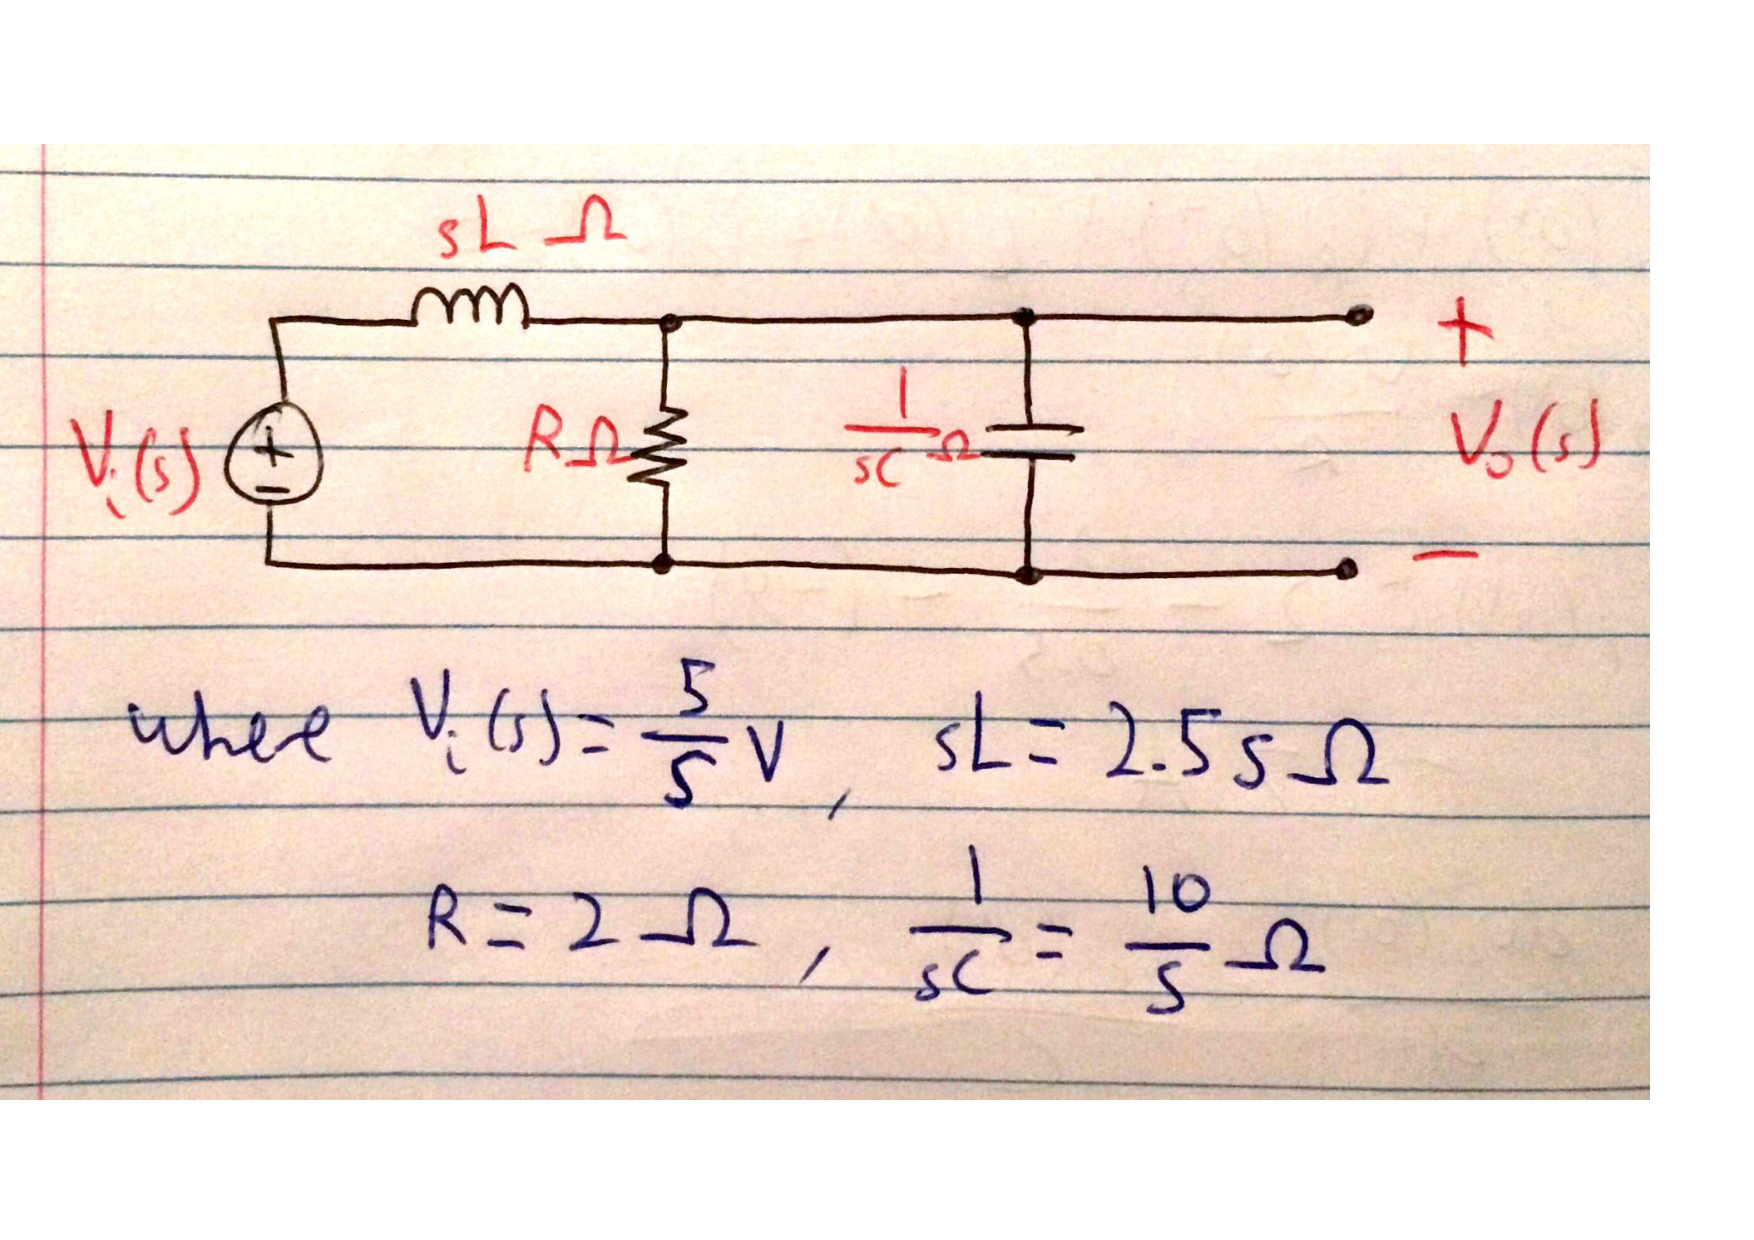
\includegraphics[scale=0.55]{q2a.pdf}
		\end{figure}
		The circuit is a voltage divider:
		\begin{align*}
			V_o(s) &= V_i(s) \times \frac{Z_R || Z_C}{Z_R || Z_C + Z_L} \\
			&= \frac{5}{s} \times \frac{\frac{20s}{s(2s+10)}}{\frac{20s}{s(2s+10)}+2.5s} \\
			&= \frac{5}{s} \times \frac{1}{1+0.125(2s^2+10s)} \\
			&= \frac{5}{s(0.25s^2+1.25s+1)} \\
			&= \frac{20}{s(s+4)(s+1)}
		\end{align*}
		Perform partial fraction expansion:
		\begin{equation*}
			\frac{20}{s(s+4)(s+1)} = \frac{A}{s} + \frac{B}{s+4} + \frac{C}{s+1}
		\end{equation*}
		\begin{equation*}
			\therefore 20 = A(s+4)(s+1) + Bs(s+1) + Cs(s+4)
		\end{equation*}
		Now solve for A, B and C:
		\begin{equation*}
			s = 0 \implies 20 = A(4)(1) \implies A = 5
		\end{equation*}
		\begin{equation*}
			s = -4 \implies 20 = B(-4)(-3) \implies B = \frac{5}{3}
		\end{equation*}
		\begin{equation*}
			s = -1 \implies 20 = C(-1)(3) \implies C = -\frac{20}{3}
		\end{equation*}
		And we arrive at $V_o(s)$ in partial fraction expanded form:
		\begin{equation*}
			V_o(s) = \frac{5}{s} + \frac{5}{3(s+4)} - \frac{20}{3(s+1)} \ \mathrm{V}
		\end{equation*}
		\\
	}
	\item{
	%Part b
		Perform the inverse Laplace transform:
		\begin{align*}
			v_o(t) &= \mathcal{L}^{-1}\left[ V_o(s) \right] \\
			&= \left(5 + \frac{5}{3}e^{-4t} - \frac{20}{3}e^{-t} \right) u(t) \ \mathrm{V}
		\end{align*}
		\\
	}
	\item{
	%Part c
		We need to develop a more detailed s domain model of the capacitor when we assume it has a non zero voltage across it at $t=0^-$:
		\begin{equation*}
			i_c(t) = C \frac{\mathrm{d}v_c(t)}{\mathrm{d}t}
		\end{equation*}
		Take the Laplace transform of both sides:
		\begin{align*}
			\mathcal{L} \left[i_c(t) \right] &= \mathcal{L} \left[C \frac{\mathrm{d}v_c(t)}{\mathrm{d}t} \right] \\
			I_c(s) &= C \left(sV_c(s) - v_c (0^-) \right) \\
			&= sCV_c(s) - CV_{c_o}
		\end{align*}
		Where $V_{c_o}$ is the voltage across the capacitor at time $t=0^-$.
		\\ \\
		The diagrammatic representation of this is a capacitor parallel to a current source whose direction is opposite to the reference current direction through the model at its terminals:
		\begin{figure}[H]
			\centering
			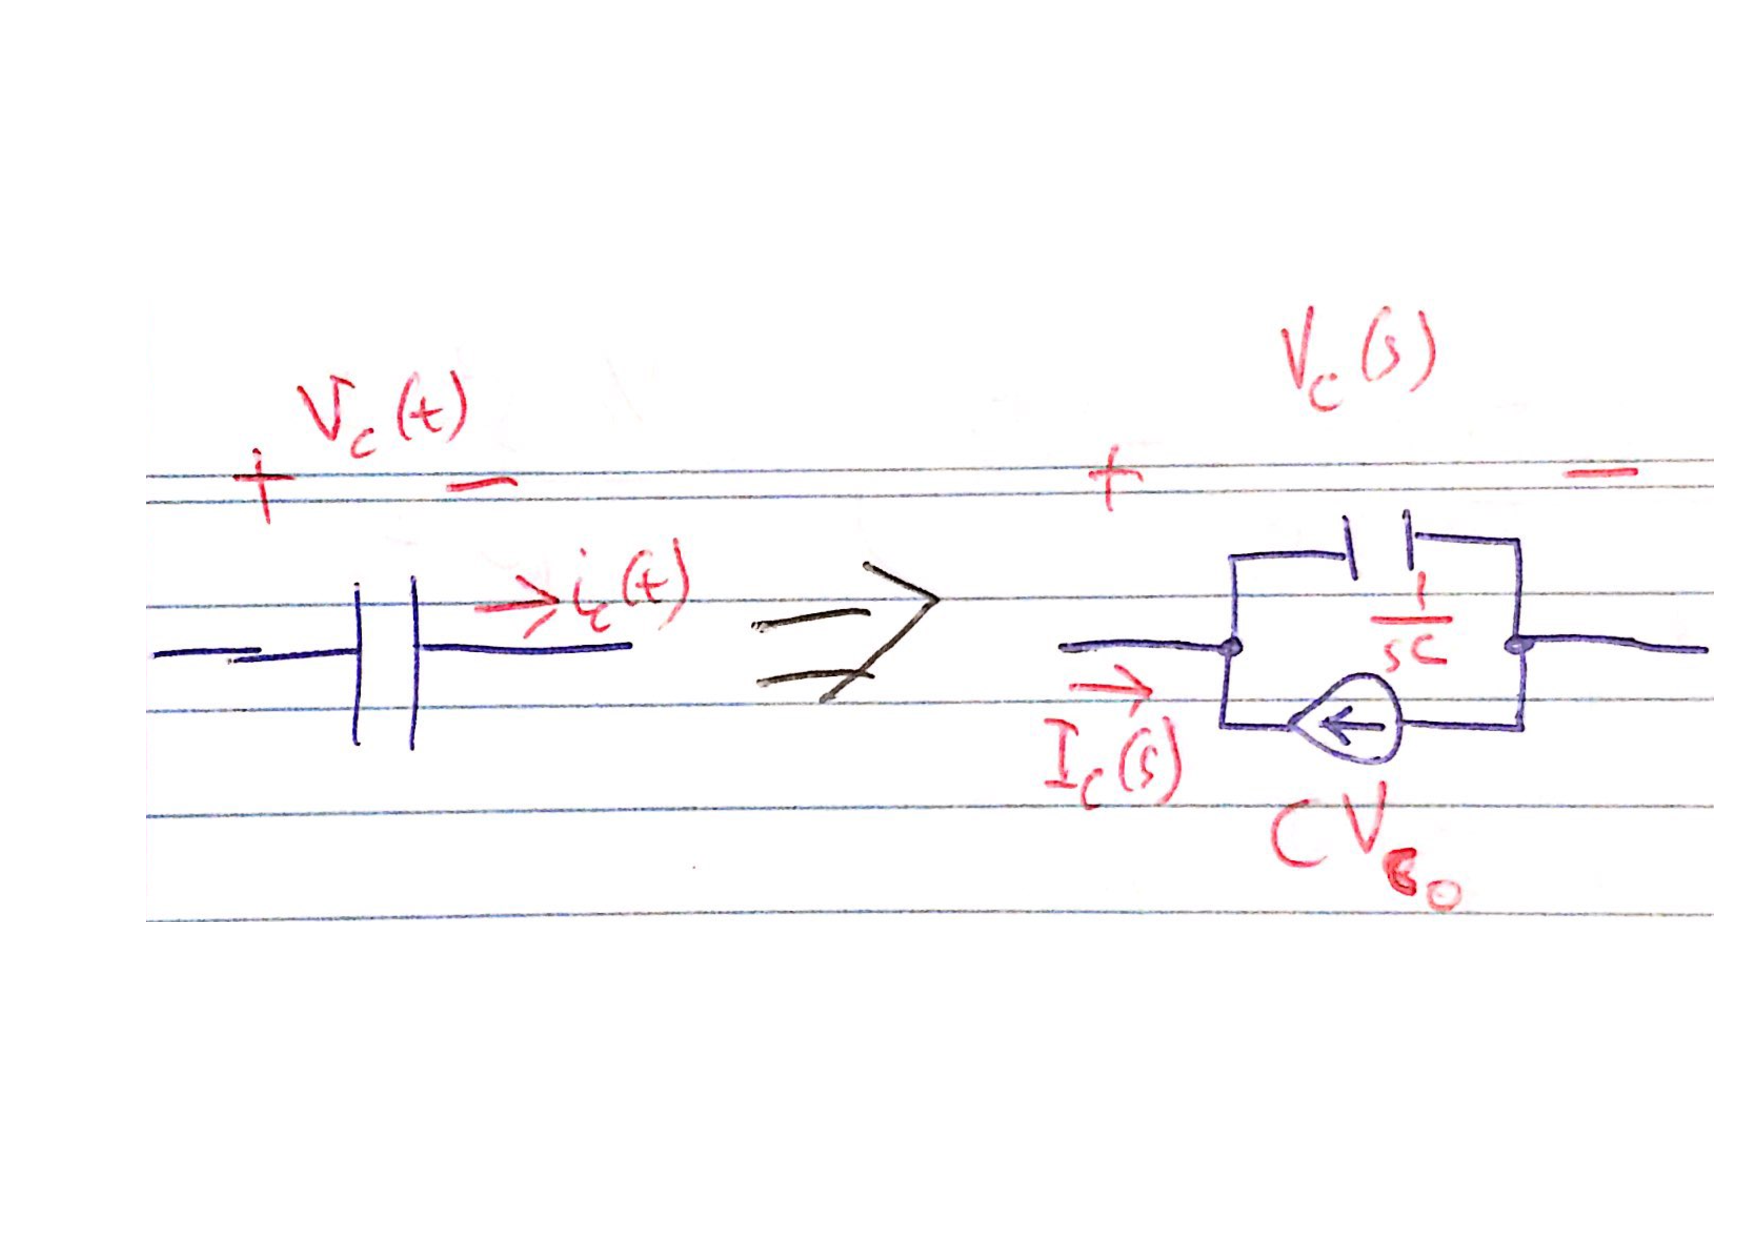
\includegraphics[scale=0.5]{q2c1.pdf}
		\end{figure}
		We substitute this new capacitor model into the original s domain diagram of the circuit:
		\begin{figure}[H]
			\centering
			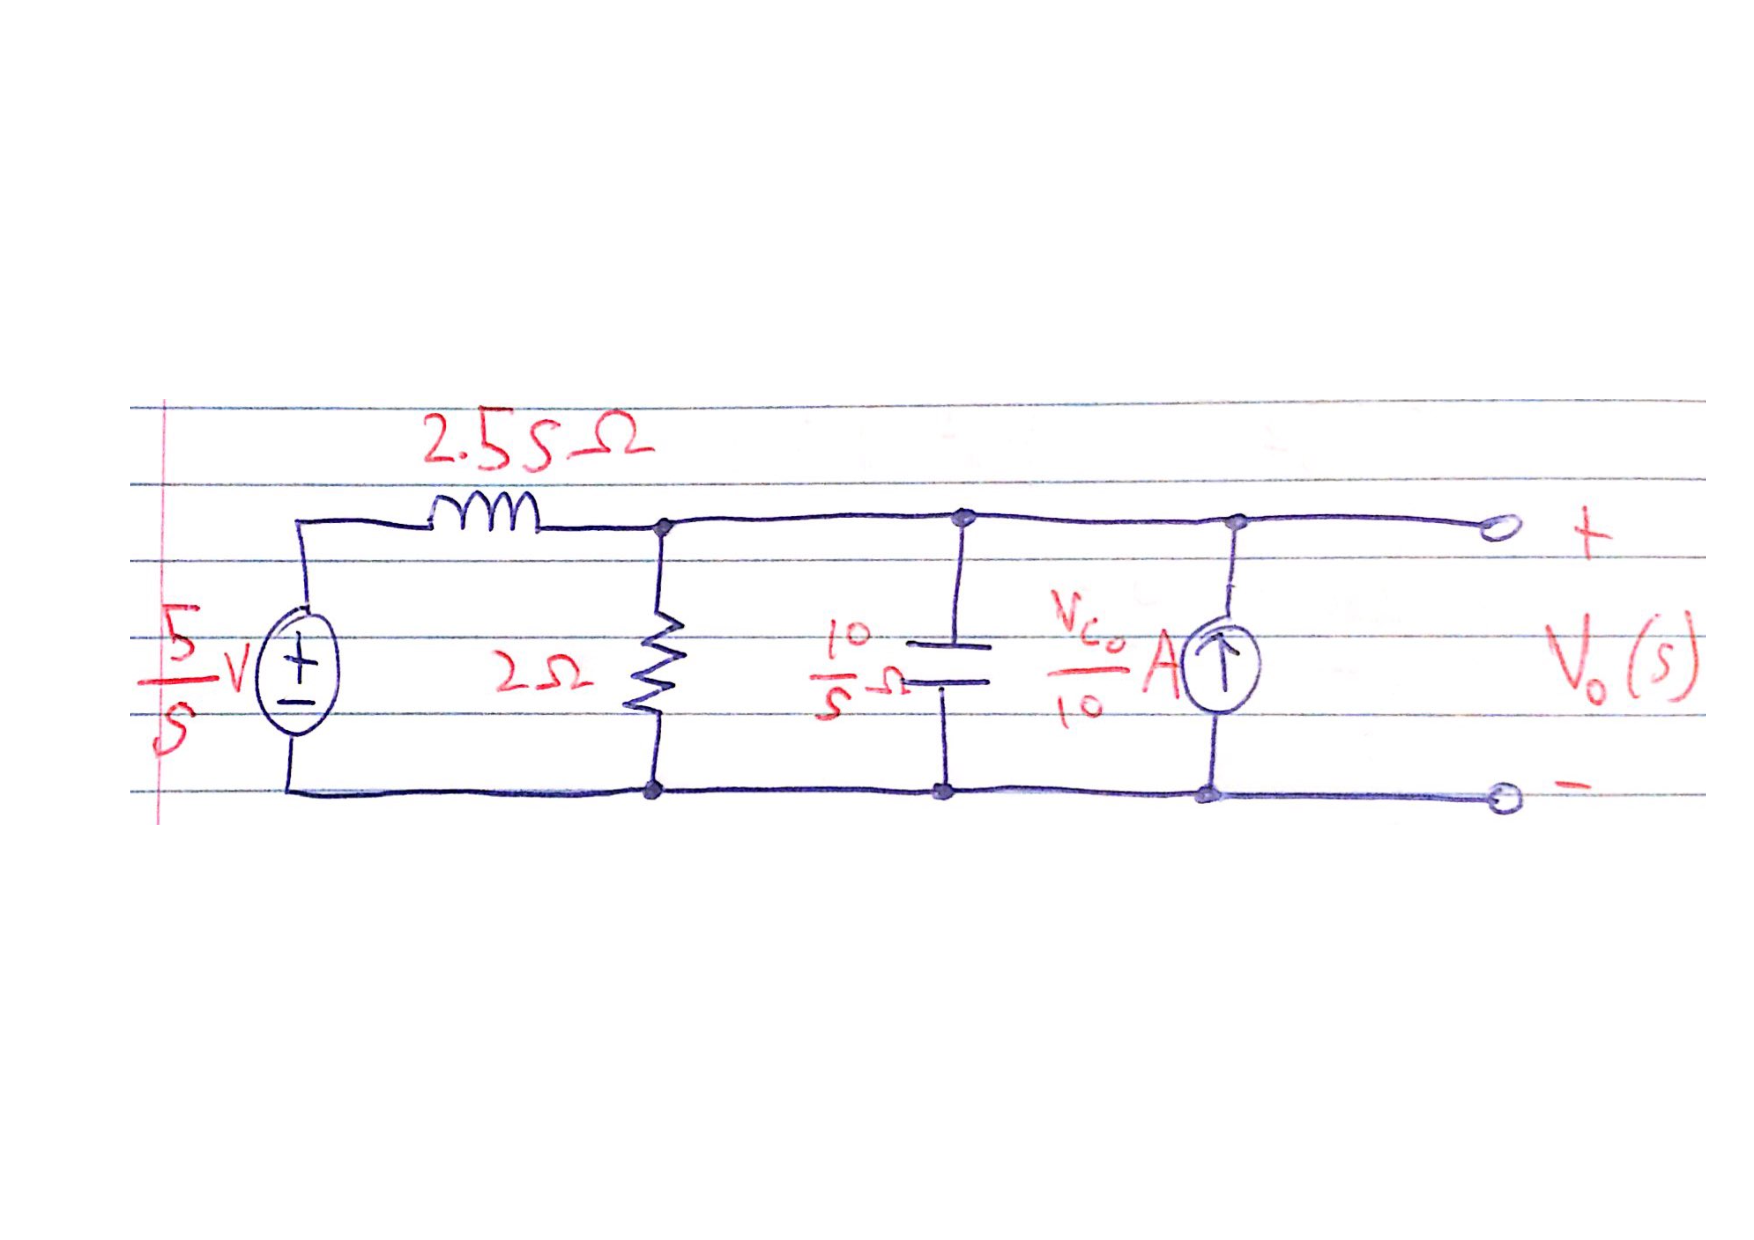
\includegraphics[scale=0.5]{q2c2.pdf}
		\end{figure}
		We perform node voltage analysis to find $V_o(s)$:
		\begin{equation*}
			\frac{V_o(s) - \frac{5}{s}}{2.5s} + \frac{V_o(s)}{2} + \frac{s \cdot V_o(s)}{10} - \frac{V_{c_o}}{10} = 0
		\end{equation*}
		Take all constants to right hand side and factor out $V_o(s)$ from what remains on left hand side:
		\begin{align*}
			V_o(s) \left(\frac{1}{2.5s} +\frac{1}{2} + \frac{s}{10} \right) &= \frac{2}{s^2} + \frac{V_{c_o}}{10} \\
			V_o(s) \left(\frac{5s^2+25s+20}{50s} \right) &= \frac{V_{c_o} \cdot s^2 + 20}{10 s^2}
		\end{align*}
		\begin{align*}
			V_o(s) &= \frac{V_{c_o} \cdot s^2 + 20}{10s^2} \cdot \frac{10s}{s^2 + 5s + 4} \\
			&= \frac{V_{c_o} \cdot s^2 + 20}{s (s+4)(s+1)} \\
		\end{align*}
		Perform partial fraction expansion:
		\begin{align*}
			\frac{V_{c_o} \cdot s^2 + 20}{s (s+4)(s+1)} &= \frac{A}{s} + \frac{B}{s+4} + \frac{C}{s+1} \\
			\therefore V_{c_o} \cdot s^2 + 20 &= A(s+4)(s+1) + Bs(s+1) + Cs(s+4) \\
		\end{align*}
		Now solve for A, B and C:
		\begin{equation*}
			s = 0 \implies 20 = A(4)(1) \implies A = 5
		\end{equation*}
		\begin{equation*}
			s = -4 \implies 16 V_{c_o} + 20 = B(-4)(-3) \implies B = \frac{4 V_{c_o} + 5}{3}
		\end{equation*}
		\begin{equation*}
			s = -1 \implies V_{c_o} + 20 = C(-1)(3) \implies C = -\frac{V_{c_o} + 20}{3} \\
		\end{equation*}
		Therefore we have $V_o(s)$ in partial fraction expanded form:
		\begin{equation*}
			V_o(s) = \frac{5}{s} + \frac{4 V_{c_o} + 5}{3(s+4)} -\frac{V_{c_o} + 20}{3 (s+1)}
		\end{equation*}
		It is noted that only the coefficients of the $\frac{1}{s+c}$ terms are changed by a non-zero initial voltage across the capacitor.
		\\ \\
		Specifically, the $\frac{1}{s+4}$ term's coefficient changes from $\frac{5}{3}$ to $\frac{4 V_{c_o} + 5}{3}$ i.e. its coefficient increases for increasing values of $V_{c_o}$.\footnotemark[1]
		\par
		The $\frac{1}{s+1}$ term's coefficient changes from $-\frac{20}{3}$ to $-\frac{V_{c_o} + 20}{3}$ i.e. its coefficient decreases for increasing values of $V_{c_o}$.\footnotemark[1]
		\\
	}

\end{enumerate}
\footnotetext[1]{Note that increasing here means a positive value becoming more positive or a negative value becoming less negative, and decreasing means the opposite.}

